\documentclass[a4paper,11pt,oneside]{article}

\usepackage{graphicx}

\begin{document}

\title{L'Bl\"{u}r: an Alternative to LabelMe in the World of Image Labelling Software}
\author{s0934142 \and s0901522}
\maketitle

\tableofcontents

\section{LabelMe}
LabelMe is the product offered by MIT that our system is intended to be
functionally equivalent to.  There are therefore valuable lessons, both good and
bad, to be learnt from how LabelMe has been implemented.

With regards to good design practice we can see that LabelMe is compliant with
Shneiderman's third, fourth, fifth and sixth golden rules.  The third rule
because have a list of labels by the side allowing you to see what labels have
been made, also from the good use of colour allowing you to easily see when a
object has been completely marked out.  The fourth rule because the dialogue
boxes that appear have a clear x in the top right corner which is consistent
with user's expectations, also any of the three options done, adjust and delete
close the dialogue.  The fifth and sixth of Schneiderman's rules we see as
fairly interlinked.  There is support for deleting an object, adjusting an
object and undoing one's actions.  This gives us easy reversal of actions and
support for error handling.

LabelMe also obeys principles 1, 5, 7 and 10 of Nielsen's usability heuristics. 
heuristic one is acheived by displaying the labels that have been added and by
adding a transluscent layer over all marked objects allowing a user to tell at a
glance what they have achieved.  Heuristic 5 is achieved in the same as way as
Shneiderman's fifth golden rule.  Heuristic 7 is acheived by using icons which
are self explaniatory and by having a simple process to control the application,
 i.e. that you do not have to remember combinations of key presses to do
anything. Heuristic 10 is acheived by having a clear help icon seen at all
times, this ties in with 7 by using a question mark which is a universal
standard for software help.

However it is not all good as we have breaches of Shneiderman's first and
second golden laws and Neilsen's ninth heuristic.  The first golden law is
breached because the erase button is actually an undo button, this mislabelling
could be prevented if the text labels were removed leaving only the icons.  
Although to keep consistent with the rest of the operating system a back arrow 
would be more useful, but the eraser is consistent with application's aesthetic.  
This leads us onto the breach of Neilson's 9th heuristic, although the system 
is minimalist, it is definitely not aesthetically pleasing: elements of the UI 
appear unconnected, icons are unevenly spaced and iconsistent in design with 
the erase button not having a red outline, and on a more subjective level we 
do not like the cartoony style of its design.  Shneiderman's second law is 
breached by there not being any short cuts for power users, these could include 
undo.

In terms of learnability, flexibility and robustness labelme is fairly good. 
It appears to be easy for new users to get to grips with learning the tool, and
can be labelling images very quickly.  Users can see their progress and easily
determine when they have successfully labelled an image.  Flexibility wise
labelme is not very flexible but it does not need to be.

Ultimately labelme is perfectly functional and easy to use, although it could be
improved in a few areas.  Its biggest problem is that it isn't pretty.  This
gives a good starting point for the development of our own image labeller, we
have assessed what works well, what doesn't and what is missing.

\section{Formal Requirements}

From analysing the mark scheme we were able to identify the following as
required functionality:
\begin{itemize}
\item Allow annotation of different images
\item Add, edit and delete labels
\item Allow saving and loading of labels
\item The above need to be easy to perform
\item Everything should follow HCI principles
\end{itemize}
The functional aspects of these requirements are not difficult to implement so
the challenge, and where we spent most of our time, was to fulfill the softer
requirements by making them easy to use and follow the principles.

GOMS

\section{L'Bl\"{u}r}

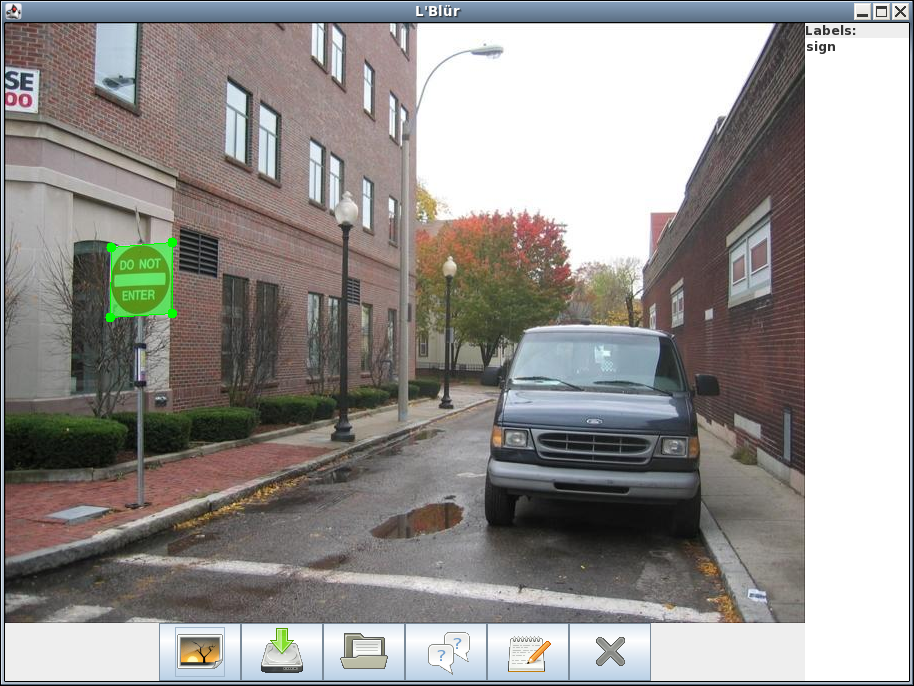
\includegraphics[width=\textwidth]{final.png}
This is the finished product.

\subsection{Design and Process}
Our design process was to iteratively build backend functionality and then make
it accessible through the frontend.  And throughout the whole process we would
fix bugs and tweak the UI.  To start with we implmented opening new images,
adding labels and saving and loading.  We then added ways to access this
functionality i.e. buttons.  We then started adding more functionality such as
adding and deleting labels.  During this we refined the previous functionality
and the user interface, so we fixed bugs that would attempt to load non existant
files causing the program to crash, and we made it more user friendly by
features like shading in marked areas and adding in right click menus.  This
cycle continued, we started to see less backend functionality be added in the
cycles and spent more time bug fixing it, but more and more coming into the
front-end with the addition of keyboard shortcuts for example.

We feel that this was an effective design discipline that let us build up a
solid product rather than focusing to heavily in one area.


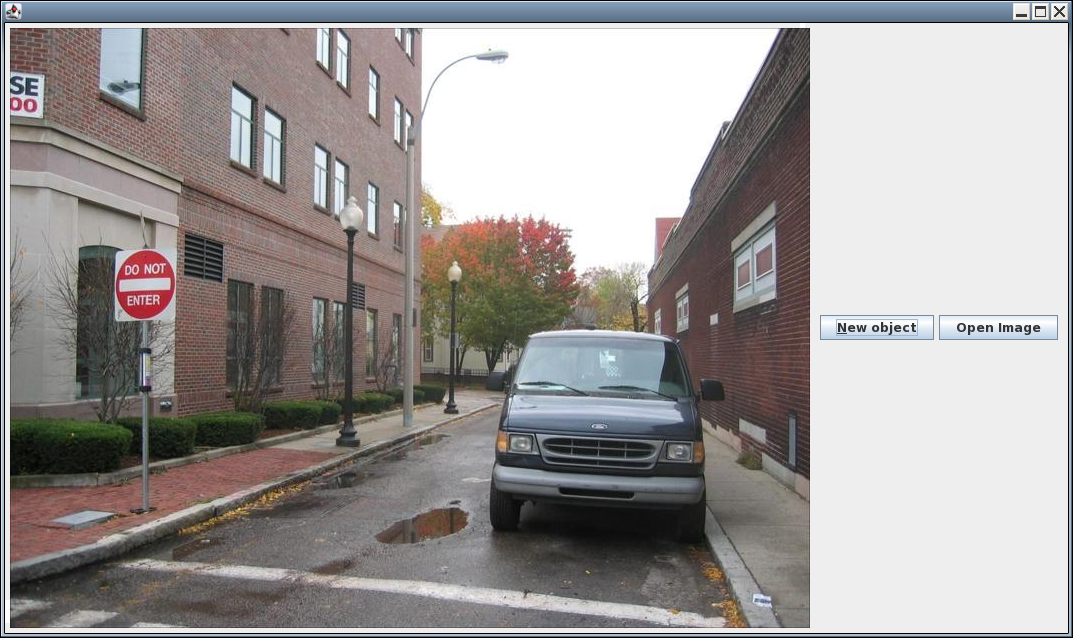
\includegraphics[width=\textwidth]{old1.png}

Our first version just added the ability to load new images.

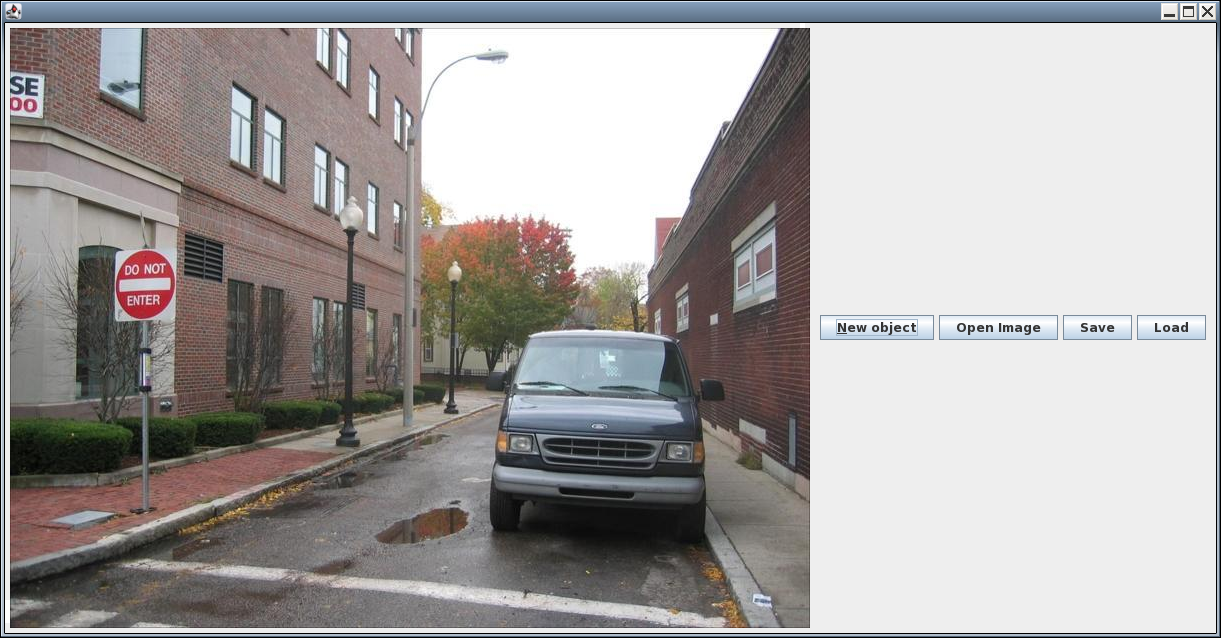
\includegraphics[width=\textwidth]{old2.png}

We then added saving and loading.

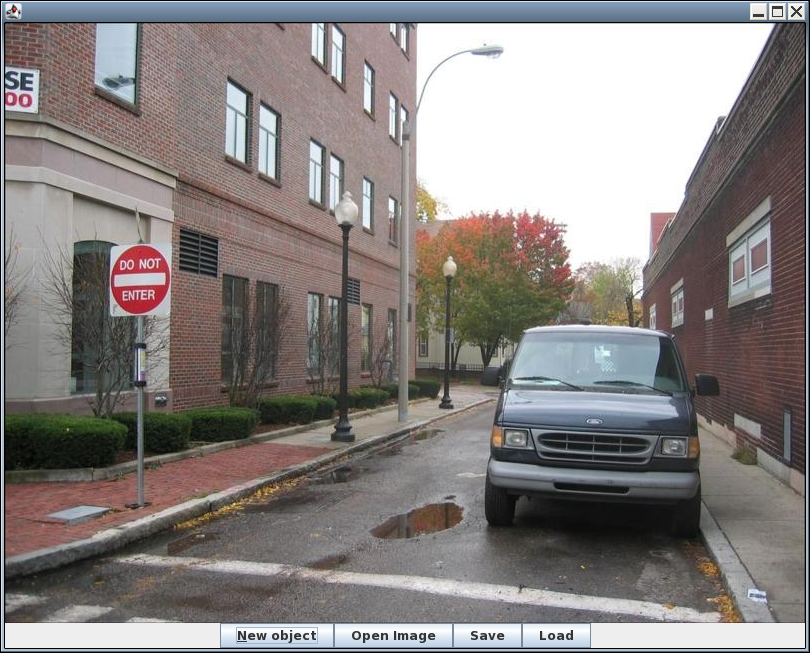
\includegraphics[width=\textwidth]{old3.png}

The buttons were starting to look very ugly by the side.  So we moved them to
be below the image.

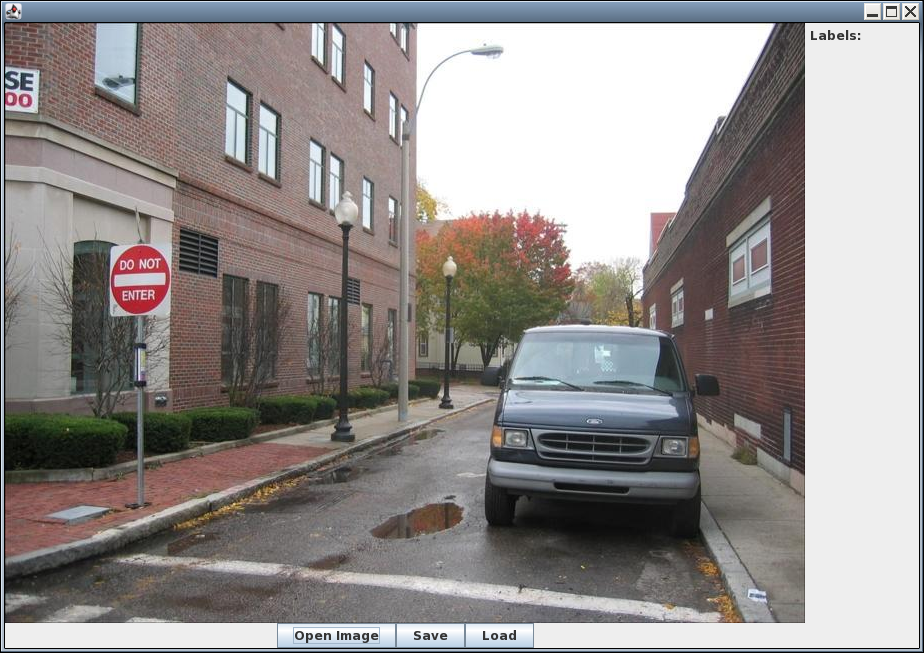
\includegraphics[width=\textwidth]{old4.png}

We then made it so you clicked on the initial node to finish a shape, so we
removed the new object button.

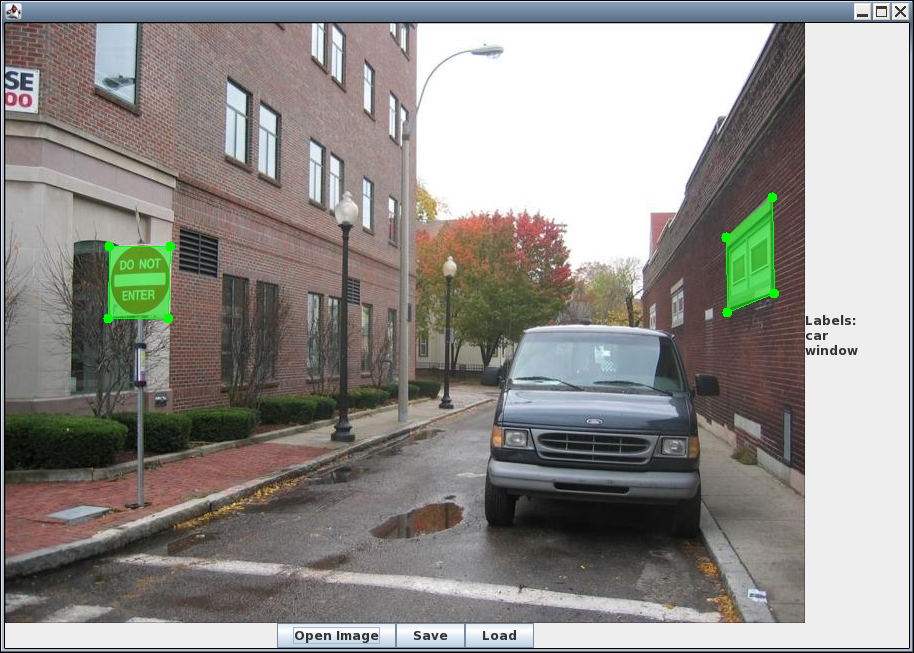
\includegraphics[width=\textwidth]{old5.png}

Then we added a label bar on the side which displayed each label as a JLabel.

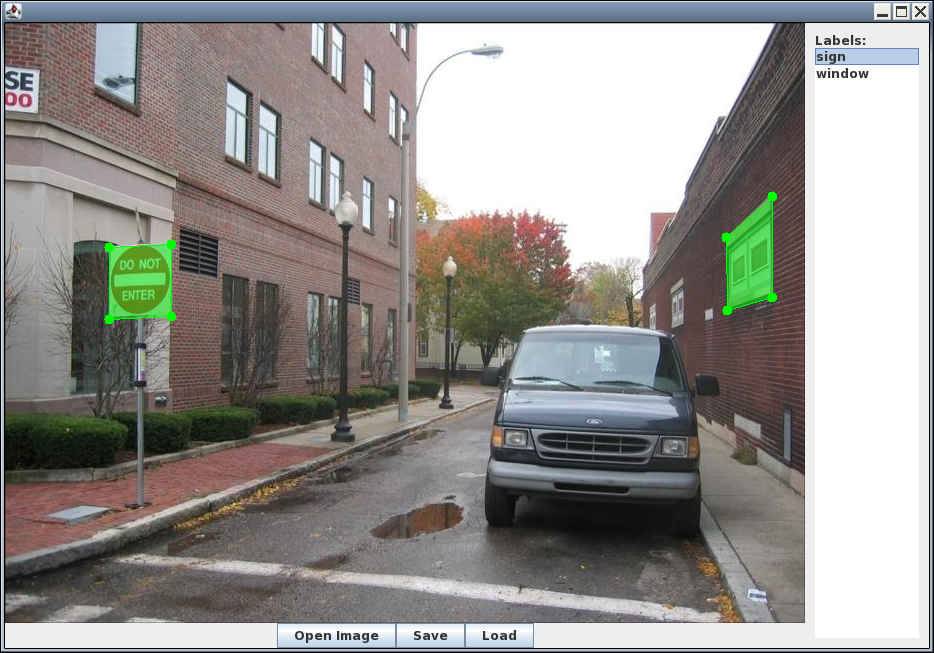
\includegraphics[width=\textwidth]{old6.png}

This was not the nicest way of displaying labels so we switched to using a list
box.

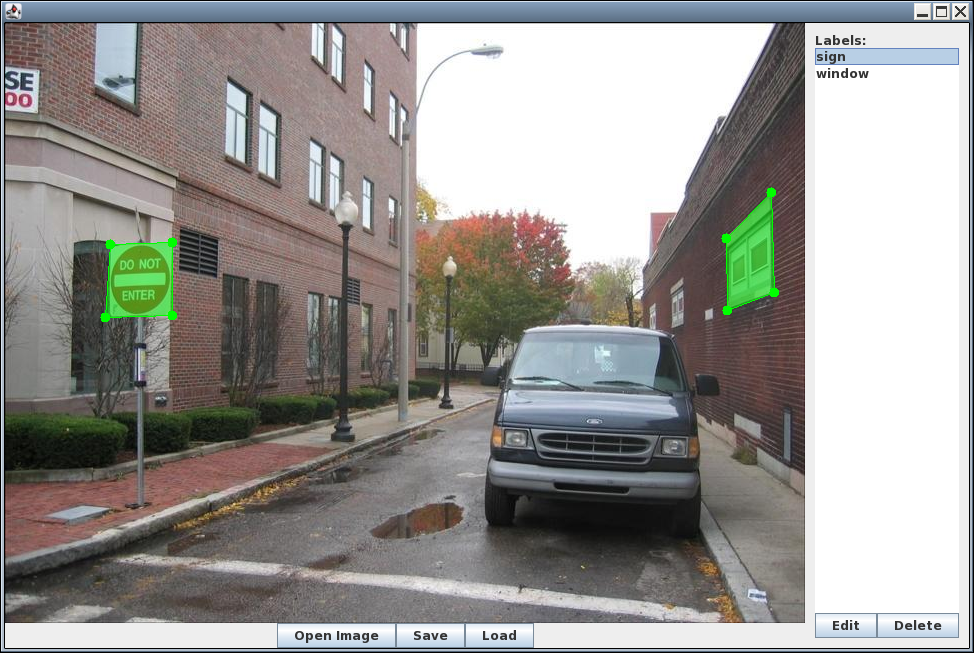
\includegraphics[width=\textwidth]{old7.png}

Then we added editing and deleting.

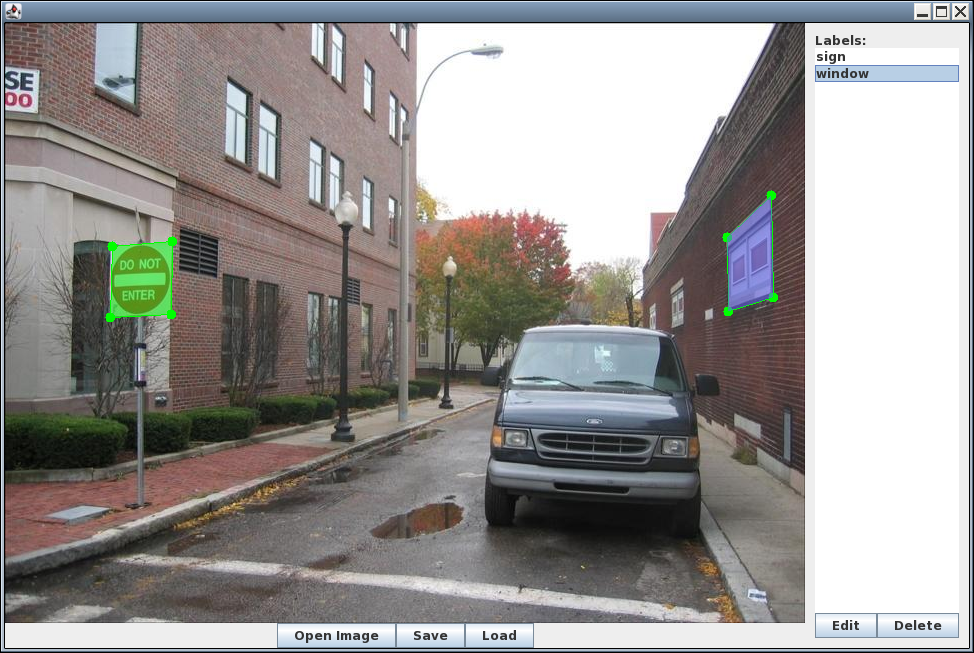
\includegraphics[width=\textwidth]{old8.png}

We then made it so the selected object is highlighted blue.

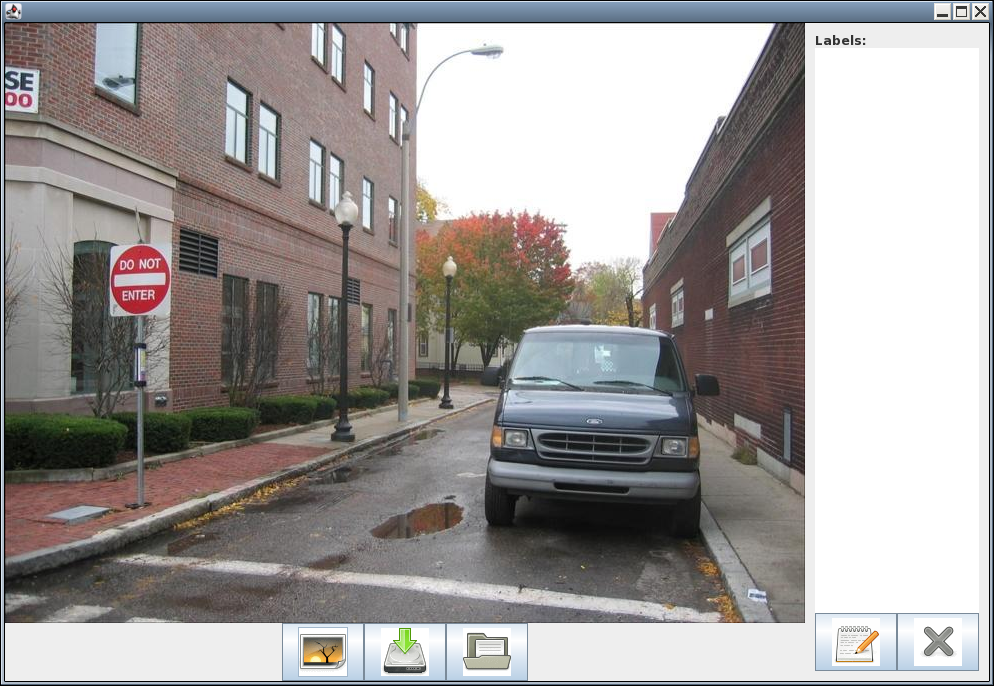
\includegraphics[width=\textwidth]{old9.png}

We then switched to using icons.

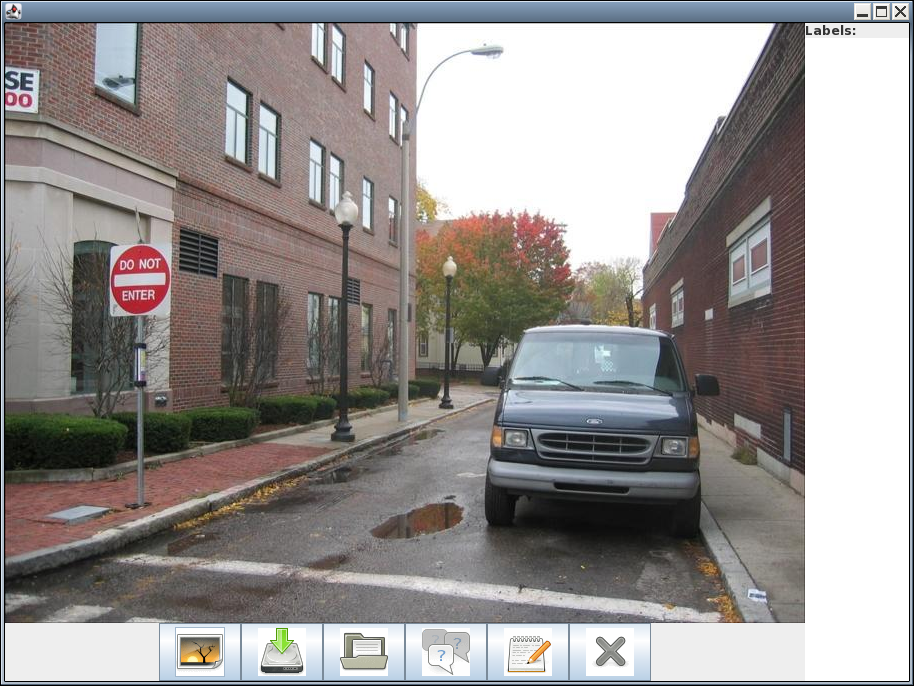
\includegraphics[width=\textwidth]{old10.png}

Then we put all the buttons together which made the UI look much nicer.

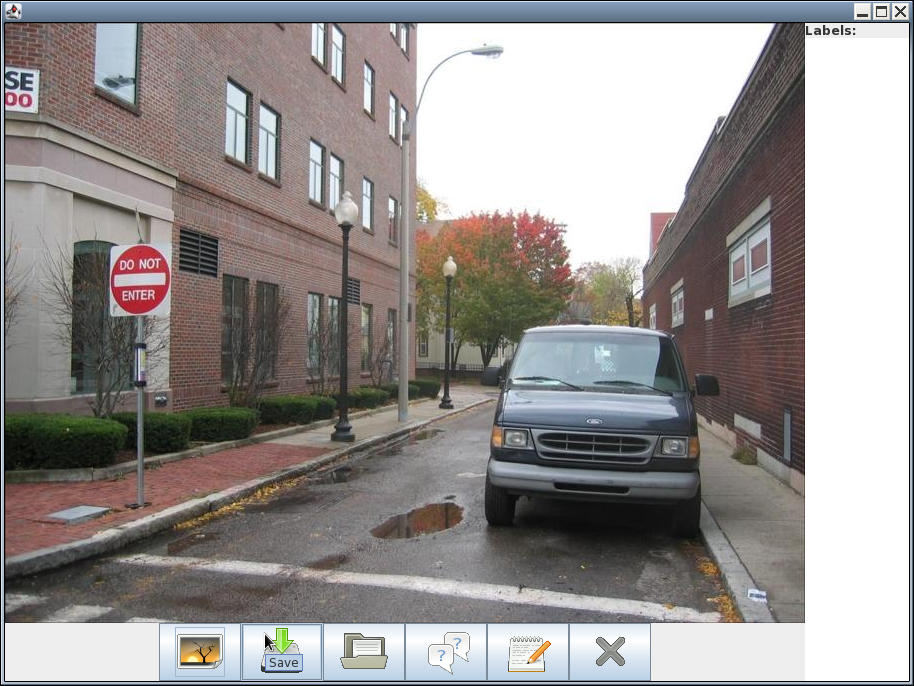
\includegraphics[width=\textwidth]{old11.png}

Finally we made the icons transparent and added tooltips.

\subsection{The Good}

\subsubsection{Saving and Loading}
We made the decision that marked points and labels would be stored in an XML
file.  This is because XML is good for storing structured data which is what we
have.  It also means it is in a semi standard format which would hopefully make
it easier if any other labelling software wanted to be used, for example LabelMe
which also has xml capability.  Although XML is a human readable format, this is
less a benefit to the user and more a benefit any researchers who want to access
the data.

Another decision we made was to not give the user much control over saving and
loading.  When you save after doing some marking and labelling the xml file is
created in the same directory as the image with the name
\emph{imagefilename}.xml.  Then when you press load after opening a new image
the relevant file is automatically loaded.  We chose to do this to simplify the
process for the user, they have to deal with fewer menus and they don't have to
remember where they saved the data.

The only downside is that the directories may start to become cluttered with
.xml files.  Which has the potential to annoy some users.  We did consider
making the xml files hidden.  This visually solves the clutter problem but
makes it harder for any user without some command line knowledge to delete old
label files.  For this reason we decided to keep them visible.

Because the actual saving and loading happens behind the scenes it is important
to inform the user that things have happened.  When a user saves their work a
modal dialogue opens on completion informing them that the save has been
successful. When a user loads a file, if no file exists they are informed via a
dialogue that there was nothing to load, otherwise nothing would happen and this
could confuse them.  If the load is successful a modal dialogue reassures the
user, in addition to the visual confirmation because of objects and
labels appearing on screen. Likewise when a new image is opened the change in
image offers confirmation that it has worked.

\subsubsection{Marking Objects}
In the example code provided if you wanted to complete the marking of an image
you had to press a button on the GUI.  This was clunky and very unintuitive.  It
makes far more sense that to complete the marking you just click on the original
node to finish it.  So this is what we implemented.

\subsubsection{Undo}
An undo feature is a fundamental aspect of almost all applications in which
a user interacts with.  It allows them to fix any mistakes they might make.  We
have our undo which is able to undo back to the last completed object.  It would
be nice to allow the user to undo back to the start, but unfortunately this is
not possible at the moment it would definitely be something we would look into 
including if we had more time.  You can however delete completed objects, 
allowing you to go back to having a clean slate if you want.  The undo method
is called with a right mouse click keeping it consistent with applications like
MSPaint.  It also means that control is kept simple and a user does not need
to locate something on the GUI, or take their hand off the mouse.

\subsubsection{Icons}
Icons are important in an application because they inform a user as to what will
happen without having to read text.  We are using the gnome tango icon set in
our application.  We order these actions from left to right in a logical order
of use: loading an image (starting a project) saving, loading a save, adding
labels and deleting objects. The latter two are deliberately nearest the label
list on the right in order to have them in easy reach. Our early prototype
systems had these controls in the right hand panel itself, but it was decided a
unified and centralised location for all controls helped the coherence of the
application.

\subsubsection{Keyboard Shortcuts}
Keyboard shortcuts were identified as an essential component to improve
experience once a user has reached a stage of familiarity with the task, as per
Schneiderman's second golden rule.  In L'Bl\"{u}r these are learnt during the
investigative phase via tooltips that appear when hovering the mouse over the
GUI buttons. Although the user requires the mouse to plot the polygons on the
image, the keyboard can be used effectively and rapidly to fulfil the remaining
application functions. Once the user has added points, pressing the right arrow
on the keyboard will bring focus to the label list, allowing the user to edit or
delete the polygon with the keyboard. Navigating up and down this list to change
selection is achieved with the arrow keys.

\subsubsection{Visual Feedback}
When an item in the labels list is selected (by mouse or keyboard) the
corresponding region on the image is highlighted in blue, matching the blue
used in the list. This also occurs in reverse; selecting the polygon for label
editing (by right-clicking the shape) also paints it blue in both locations.
The consistency ensures intuitive behaviour and allows the user to get instant
feedback on whether they have selected the correct shape/label.

\subsection{The Bad}

\subsubsection{Screen Flicker}
Currently there is quite bad screen flicker from having the image redrawn.  This
occurs when the window is moved partially offscreen or when dialogue boxes are
moved.  This is a very annoying thing to happen and substantially degrades the
user experience. Any version of the software released to end users would
definitely require a solution to this.  We believe the way to fix this problem
would be to perform double buffering; a process where the image is processed in
one buffer and then put directly into another buffer to be displayed.  If we
were to implement double buffering it would provide the user with a far smoother
experience.

\subsubsection{Label Dialogue Boxes}
At the moment dialogue boxes relating to adding/editing of labels all are
spawned at the same point: The centre of the user's monitor.  It would be much
more desirable to have them be more like tooltips appearing next to the marked
area.  This would give the user more confirmation about what they are editing.

\subsubsection{No Easy Way to Change Marked Objects}
Currently once you have finished marking out an object if you decide you want to
change it the only way to do this is by deleting the object and re-marking it.
This is very awkward and it would be an area we looked into if we had more time.
Allowing the user to add new nodes to an object would probably be infeasible, 
but we could let the user click and drag existing nodes to alter the shape.  
This would be a feature aimed more at advanced users as it would allow for a
greater throughput when labelling images.  To the casual user it wouldn't matter
as much we feel.

\subsection{The Ugly}
\subsubsection{General Aesthetic}
A fundamental part of HCI design is that interface be aesthetically pleasing and
minimal (Neilson - 9).  We feel that we have achieved the minimal part of that,
but not the aesthetically pleasing part.  Swing is not the prettiest thing in
the world.  If we had more time we would look into finding a nice theme to use
and applying it.  This would make the program more appealing to use to users.

\subsection{Improvements}
The following are features that we identified as useful additions and would have
liked to implement but ran out of time.

\subsubsection{A Gallery of Pictures} 
Having something like a bar along the bottom that displays all the images in the
current directory.  This is good for the user as it means they do not have to
keep navigating the file dialogue when they want to start labelling a new image
in the same directory (recognition not recall, and reduces load on short term
memory).  It also would add colour to the UI making it more attractive. If the
goal of the program is to label images en masse, perhaps a simple arrow to
navigate back and forward (as in an image preview application) would speed the
process significantly.

\subsubsection{A Gallery of Labels}
Instead of just having a list of the text of labels that have been added to an
image we would like the section of the image marked out for labelling to appear
in a gallery as an icon for that label.  In cases where there are ambiguous
labels, or many objects with the same/similar labels as rather than a user
trying to remember which label corresponds to which object, or attempting trial
and error to find the match, instead the user would just be able to match areas
of the picture with the icons, giving them a much smoother interaction with the
system.  This could be combined with the gallery of pictures mentioned above and
allowing the user to tab between the two views, this would help keep the
application consistent.

\subsubsection{Changing the Colour of Marked Objects}
Although the program can handle stacking shapes, it would be more useful to
change the on-screen colour of each shape, and tying it to the label colour in
the list.  This would allow the stacked shapes to be far more easily distinguished,
much improving the user experience. Highlighting the shape in this case could
darken or lighten the colours.

\subsubsection{Scaling}
The software currently only handles images at 800 x 600 pixels in size;
larger images that are loaded will only be partially visible, and smaller
images are shunted to the top corner of the interface. Ideally the image would
be resized to fit the window size - this would help appearance as well as
usability.


\subsection{Conclusion}
L'Bl\"{u}r improves upon LabelMe with greater adherence to both Shneiderman's
Golden Rules and Nielsen's 10 Usability Heuristics - for example,
the inclusion of shortcuts and improved design consistency. The feedback
dialogues, undo feature and error handling also help conform to each set of
guidelines.  In terms of learnability we feel that like LabelMe we do not
require much learnt knowledge.  A user should be able to come in and set 
straight to labelling and if they do get stuck then there is a help feature to
guide them, this is a low cognitive load for the user which is preferable.
In terms of flexibility we feel we are better than LabelMe, we have
the same range of ways in which information is shared between program and user
but we have given the user a range of control options with the addition of
keyboard shortcuts.  In terms of robustness we feel we are on the same level as
LabelMe.

\section{Appendices}
\appendix

\section{Shneiderman’s 8 Golden Rules (1987)}
\begin{enumerate}
\item Strive for consistency
\item Enable frequent users to use shortcuts
\item Offer informative feedback
\item Design dialogs to yield closure
\item Offer error prevention and simple error handling
\item Permit easy reversal of actions
\item Support internal locus of control
\item Reduce short-term memory load 
\end{enumerate}

\section{Nielsen’s 10 Usability Heuristics (1994)}
\begin{enumerate}
\item Visibility of system status
\item Match between system and the real world
\item User control and freedom
\item Consistency and standards
\item Help users recognize, diagnose and recover from errors
\item Error prevention
\item Recognition rather than recall
\item Flexibility and efficiency of use
\item Aesthetic and minimalist design
\item Help and documentation
\end{enumerate}
\end{document}
